\chapter{Adders}
\label{ch:adders}\

%%\textit{ripple-carry adders, twos complement, subtraction, \dots}

\section{Adding Numerals}
\label{sec:addition-by-numeral}

When people do paper-and-pencil
\index{arithmetic!paper and pencil}arithmetic,
they use decimal numerals.
For example, to add two numbers, a person
writes down the decimal numerals for the numbers,
one under the other with the digits lined up so that
the units digit of one number is directly under
the units digit of the other, and similarly for
the tens digits, hundreds digits, and so on.
Then, the units digits are added together,
and the low-order digit of that sum is written
below the units-digit column.

\begin{figure}
\begin{center}
\begin{minipage}[b]{0.4\textwidth}
\begin{verbatim}
   11 1    carries
    ----
    9542   first addend
  +  638   second addend
    ----
   10180   sum
\end{verbatim}
\end{minipage}
\end{center}
\index{numeral!addition}\index{addition!decimal numeral}\index{arithmetic!decimal numeral}
\caption{Adding Decimal Numerals}
\label{fig:adding-decimal-numerals}
\end{figure}

If the sum of the units digits is ten or more, a
\index{carry, addition}\index{addition!carry}carry
is marked above the tens-digit column.
Then, the sum of that carry (if there was one) and
the tens digits is computed.
As before, the low-order digit of the sum
goes into the numeral, this time in the
tens-digit column, and the carry,
if there was one, is marked
above the hundreds digit column.
This process moves across the digits of the addends until all the digits
are accounted for (Figure~\ref{fig:adding-decimal-numerals}).

To add decimal numerals in this way, a person needs to know
the table for one-digit sums (0+0=0, 0+1=1, \dots 2+2=4 \dots 9+8=17, 9+9=18).
To add binary numerals, a similar table of one-bit sums is needed,
but the table is much smaller for binary numerals
than for decimal numerals because it only has to account for
two kinds of bits ($0$ and $1$), not ten digits ($0$, $1$, $2$, \dots $9$).
The process of adding numerals is in other respects
the same for binary numerals as for decimal numerals
(Figure~\ref{fig:adding-binary-numerals}).
The small size of the table for one-bit addition simplifies
both the pencil-and-paper process and the design of
digital circuits for addition of binary numerals, compared to
designing circuits for decimal numerals.\footnote{The table
in Figure~\ref{fig:adding-binary-numerals}
relies on commutativity and associativity
(Figure~\ref{fig-02-02}, page \pageref{fig-02-02})
for completeness.}

\begin{figure}[!tbp]
\begin{center}
\begin{minipage}[b]{0.4\textwidth}
\begin{verbatim}
   11 111 1    carries
    --------
    01011101   first addend
  + 11010101   second addend
    --------
   100110010   sum
\end{verbatim}
\end{minipage}
\hfill
\begin{minipage}[b]{0.4\textwidth}
~~~~~~\emph{one-bit addition}\\
\vspace{.05 in}
\begin{tabular}{|c|c|c|c}
 \hline
 $+$      & $c$ & $s$ \\
 \hline
 $0+0$    & $0$ & $0$ \\
 \hline
 $0+1$    & $0$ & $1$ \\
% \hline
% $1+0$    & $0$ & $1$ \\
 \hline
 $1+1$    & $1$ & $0$ \\
 \hline
 $1+1+1$  & $1$ & $1$ \\
 \hline
\end{tabular}
\end{minipage}
\end{center}
\index{arithmetic!binary numeral}\index{addition!carry}
\index{numeral!binary addition}\index{addition!binary numeral}\index{binary numeral!addition}
\caption{Adding Binary Numerals}
\label{fig:adding-binary-numerals}
\end{figure}

\begin{ExerciseList}
\Exercise Describe by example the process of multiplying a pair of decimal numerals.

\Exercise Describe by example the process of multiplying a pair of binary numerals.
\end{ExerciseList}

\section{Circuits for Adding One-Bit Binary Numerals}
\label{sec:adding-1-bit-numerals}

The addition table for one-bit, binary numerals
in Figure~\ref{fig:half-adder} (page \pageref{fig:half-adder})
displays the sum as two separate bits:
a carry bit $c$ and a sum bit $s$.
A close look at the table shows that
the carry bit matches the table of values of the
digital gate for logical-and
(Figure \ref{fig-02-logic-gates}, page \pageref{fig-02-logic-gates}).
That is, the carry bit is 1 only if both inputs are 1s.
Otherwise, the carry bit is 0.
So, a logical-and gate can serve
as a digital circuit to compute the carry bit
in the addition of two one-bit, binary numerals.
Feed the signals for the one-bit numerals
into a logical-and gate, and the output signal
will represent the carry bit correctly.

Another close look reveals that the sum bit
matches the table of values of the
digital gate for exclusive-or
(XOR, Figure~\ref{fig-02-logic-gates}).
That is, the sum bit is 0 if the two inputs are the same
and 1 if they are different.
So, constructing a digital circuit to compute the sum bit
amounts to feeding the signals for the one-bit numerals
into an exclusive-or gate.
Combining these ideas for carry-bit and sum-bit circuits
leads to a two-input, two-output circuit known as a
half adder (Figure \ref{fig:half-adder}, page \pageref{fig:half-adder}).

\begin{figure}
\begin{center}
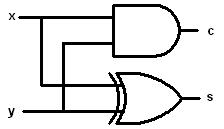
\includegraphics[scale=0.23]{Images/half-adder.png}
\todo{Improvised with PowerPoint. Redraw using Visio.}
\begin{Verbatim}
(defun and-gate (x y) (if (and (= x 1) (= y 1)) 1 0))
(defun or-gate (x y) (or (= x 1) (= y 1)))
(defun xor-gate (x y) (if (and (= x 1) (= y 1)) 0 (or-gate x y)))
(defun half-adder (x y) (list (xor-gate x y) (and-gate x y)))
\end{Verbatim}
\end{center}
\index{addition!carry}
\index{numeral!binary addition}\index{addition!binary numeral}\index{binary numeral!addition}
\index{arithmetic!binary numeral}
\index{diagram!half-adder circuit}
\index{ACL2!circuit model}\index{circuit!ACL2 model}
\index{addition!circuit}\index{circuit!addition}\index{circuit!half adder}\seeonlyindex{half adder}{circuit}
\caption{Half-Adder Circuit and ACL2 Model}
\label{fig:half-adder}
\end{figure}

Since we reason about digital circuits using the methods
of Boolean algebra, we need an algebraic representation
of the circuit-diagram for the half-adder circuit.
Remember, digital circuits are only one of four
equivalent representations of Boolean formulas that
we have studied: circuit diagrams, well-formed formulas
in the notation of mathematical logic (for example, $x \wedge y$),
Boolean formulas in engineering notation (justaposition for $\wedge$,
$+$ for $\vee$, and over-bar for $\neg$), and ACL2 notation.
The ACL2 formalization allows us mechanize some aspects of the reasoning process.
So, Figure \ref{fig:half-adder} also specifies the half-adder circuit in ACL2 terms.
We refer to this specification as an
ACL2 model of the half-adder circuit.
We use the same name for the model as the circuit:
the operator \textsf{half-adder}
delivers the two output signals as a list of two elements,
the first element being the sum bit and the second, the carry bit.

In the end, we would like to have a circuit
that adds binary numerals,
and we saw in an example (Figure \ref{fig:adding-binary-numerals})
that this would require us to deal with three input bits
in each column:
the corresponding bits in the two addends
and the carry bit brought from adding
the bits in the previous column.
The half-adder circuit is not up to this task
because it has only two input signals.
However, we can put together a full-adder circuit
by combining two half adders and a logical-or gate,
as shown in Figure \ref{fig:full-adder}
(page \pageref{fig:full-adder}).
Since the full-adder circuit has three inputs,
each of which is either 0 or 1,
there are eight possible input configurations,
as shown in the full-adder table.

\begin{figure}
\begin{center}
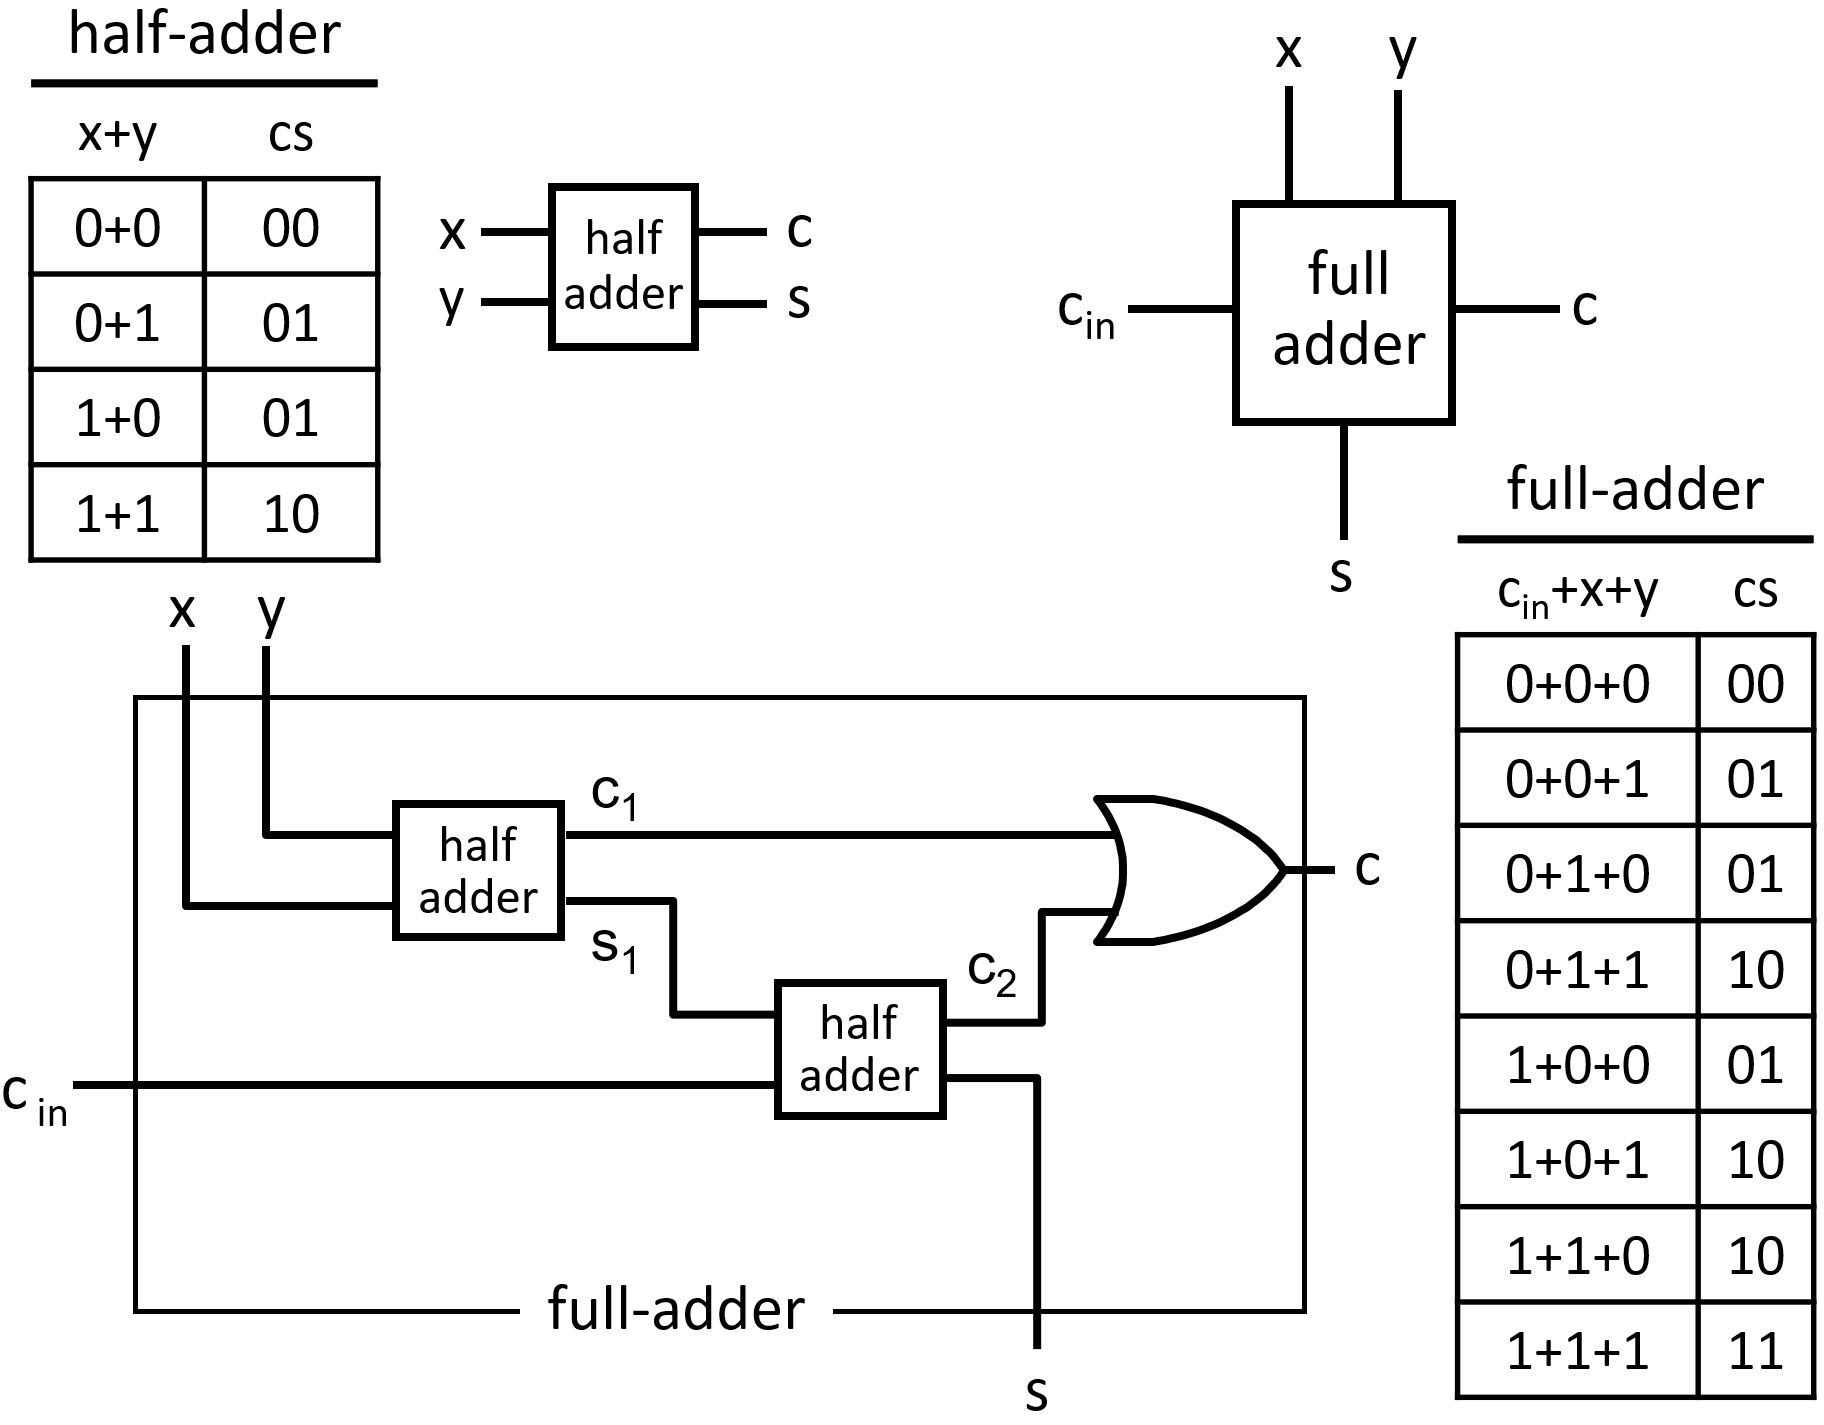
\includegraphics[scale=0.25]{Images/full-adder.png}
\todo{Improvised with PowerPoint. Redraw using Visio.}
\begin{Verbatim}
(defun full-adder (c-in x y)
  (let* ((h1 (half-adder x y))
         (s1 (first h1)) (c1 (second h1))
         (h2 (half-adder s1 c-in))
         (s  (first h2)) (c2 (second h2))
         (c  (or-gate c1 c2)))
    (list s c)))
\end{Verbatim}
\end{center}
\index{addition!carry}
\index{arithmetic!binary numeral}
\index{numeral!binary addition}\index{addition!binary numeral}\index{binary numeral!addition}
\index{diagram!full-adder circuit}
\index{addition!circuit}\index{circuit!addition}
\index{circuit!full adder}\seeonlyindex{full adder}{circuit}
\index{ACL2!circuit model}\index{circuit!ACL2 model}
\caption{Full-Adder Circuit and ACL2 Model}
\label{fig:full-adder}
\end{figure}

The \textsf{full-adder} operator defined in the figure
is a formal model in ACL2 of the circuit diagram,
and the following tests, one for each line in the table,
comprise a comprehensive, mechanized verification of
the model.

\label{full-adder-model-check}
\begin{Verbatim}
(check-expect (full-adder 0 0 0) (list 0 0))
(check-expect (full-adder 0 0 1) (list 1 0))
(check-expect (full-adder 0 1 0) (list 1 0))
(check-expect (full-adder 0 1 1) (list 0 1))
(check-expect (full-adder 1 0 0) (list 1 0))
(check-expect (full-adder 1 0 1) (list 0 1))
(check-expect (full-adder 1 1 0) (list 0 1))
(check-expect (full-adder 1 1 1) (list 1 1))
\end{Verbatim}

The \textsf{full-adder} operands
are symbols for bits, but we can use the \textsf{numb} operator
(page \pageref{nmb-defun})
to interpret them as numbers.
If $x$ is a bit, then \textsf{[$x$]} is a numeral for
the number it denotes, and the \{\emph{Horner 2}\} theorem
(Exercise \ref{horner2-thm}, page \pageref{horner2-thm})
asserts that \textsf{(numb [$x$])} computes that number.
The same theorem asserts that if $s$ and $c$ are bits,
then \textsf{(numb [$s$ $c$])} is
the number that the numeral \textsf{[$s$ $c$]} denotes.
Combining these observations with the full-adder table
(Figure \ref{fig:full-adder})
verifies the theorem \{full-adder ok\} shown in
Figure \ref{fig:full-adder-thm} (page \pageref{fig:full-adder-thm}).\footnote{The
\textsf{full-adder} operator delivers a list \textsf{[$s$ $c$]} whose first
element is the sum bit and whose second element is the carry bit.
The order of elements in the result delivered by \textsf{full-adder} was designed
to form a numeral for the sum of its three, one-bit operands.
The list in reverse order, \textsf{[$c$ $s$]},
would contain the same information,
but would not conform to our representation of binary numerals
because the low-order bit would no longer come first.}

\begin{figure}
\begin{center}
\begin{tabular}{ll}
Theorem \{\emph{full-adder ok}\} & \textsf{(numb [$s$ $c$])} $=$ \textsf{(numb [$x$])} $+$ \textsf{(numb [$y$])} $+$ \textsf{(numb [$c_{in}$])} \\
                                 & where \textsf{[$s$ $c$]} $=$ \textsf{(full-adder $c_{in}$ $x$ $y$)} \\
\end{tabular}
\begin{Verbatim}
(defthm full-adder-ok
  (= (numb (full-adder c-in x y))
     (+ (numb (list c-in)) (numb (list x)) (numb (list y)))))
\end{Verbatim}
\end{center}
\index{theorem!full adder}\seeonlyindex{full-adder theorem}{theorem}\index{theorem, by name!\{full adder-ok\}}\index{numeral!binary addition}\index{addition!binary numeral}\index{binary numeral!addition}
\caption{Full-Adder Theorem}
\label{fig:full-adder-thm}
\end{figure}

\section{Circuit for Adding Two-Bit Binary Numerals}
\label{sec:adding-2-bit-numerals}

A circuit that adds two-bit, binary numerals
comes from combining two full-adder circuits
(Figure~\ref{fig:adder2}, page \pageref{fig:adder2}).
The first full-adder circuit gets, as input, the
low-order bits, $x_0$ and $y_0$,  of the two addends.
The second full adder gets the high-order bits,
$x_1$ and $y_1$.
The circuit directs the output carry, $c_1$, from
the first full adder to the input carry of the
second full adder.

The circuit produces three output signals: one sum bit from
each full adder ($s_0$ and $s_1$) and the carry-out
from the second full adder ($c_2$).
With a carry-in of zero for the first full adder
($c_0 = 0$), the output signals form a two-bit
numeral \textsf{[$s_0$ $s_1$]} and a carry bit $c_2$
that represent the sum of the two input numerals.
More generally, the output signals
represent the sum of the two input numerals and the
carry-in bit.
The following equation \{$\star$\} shows how to interpret the
input and output signals as numbers.

\begin{center}
\textsf{(numb [$s_0$ $s_1$]) $+$ (numb [$c_2$])} $=$
\textsf{(numb [$c_0$]) $+$ (numb [$x_0$ $x_1$]) $+$ (numb [$y_0$ $y_1$])}~~~\{$\star$\}
\end{center}

\begin{figure}
\begin{center}
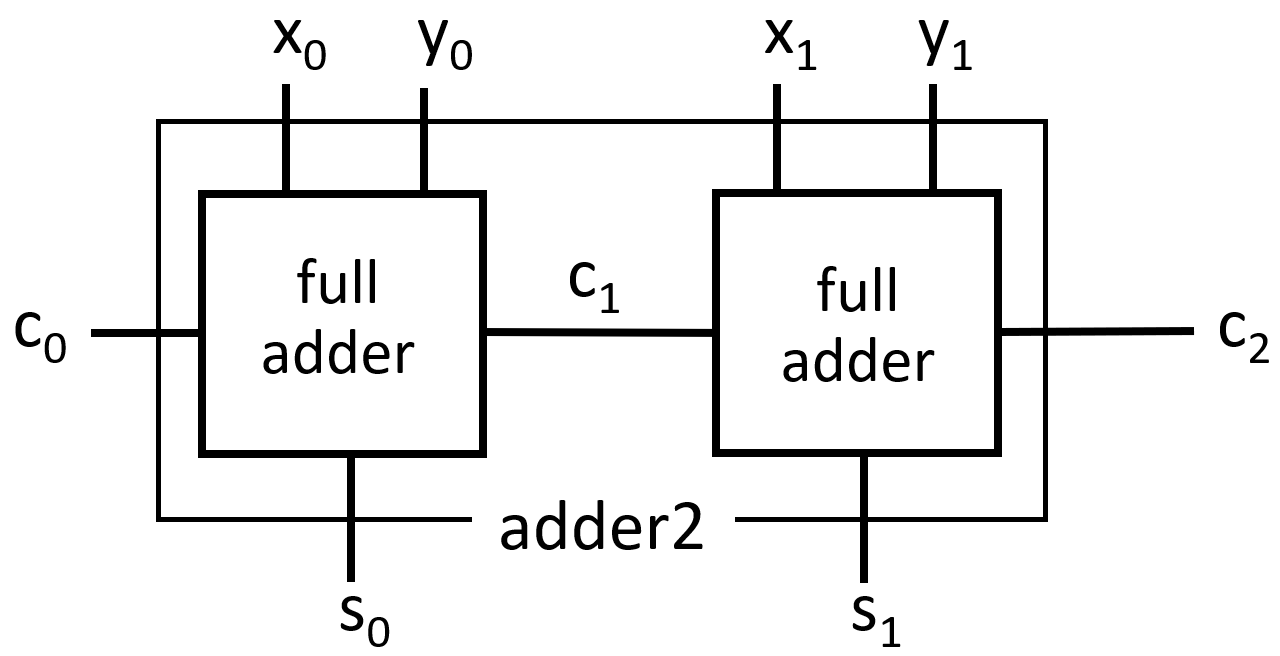
\includegraphics[scale=0.25]{Images/adder2.png}
\todo{Improvised with PowerPoint. Redraw using Visio.}
\begin{Verbatim}
(defun adder2 (c0 x y)
  (let* ((x0 (first x)) (x1 (second x))
         (y0 (first y)) (y1 (second y))
         (f0 (full-adder c0 x0 y0))
         (s0 (first f0)) (c1 (second f0))
         (f1 (full-adder c1 x1 y1))
         (s1 (first f1)) (c2 (second f1)))
    (list (list s0 s1) c2)))
\end{Verbatim}
\end{center}
\index{addition!carry}
\index{arithmetic!binary numeral}
\index{numeral!binary addition}\index{addition!binary numeral}
\index{binary numeral!addition}
\index{diagram!two-bit adder circuit}
\index{addition!circuit}\index{circuit!addition}\index{circuit!two-bit adder}\seeonlyindex{two-bit adder}{circuit}
\index{ACL2!circuit model}\index{circuit!ACL2 model}
\caption{Two-Bit Adder and ACL2 Model}
\label{fig:adder2}
\end{figure}

We refer to the output two-bit numeral, without the carry bit,
as the sum bits.
Ignoring the carry bit amounts to doing modular arithmetic, mod $2^2$
(theorem \{\emph{pfx-mod}\}, Exercise~\ref{pfx-mod}, page \pageref{pfx-mod}).

A mechanized verification of the arithmetic properties of \textsf{adder2}
could be constructed as a comprehensive sequence of check-expect tests,
as we did with the \textsf{full-adder} for one-bit addition
(page \pageref{full-adder-model-check}).
However, there would be 32 cases to check
because there are five bits of input
(a carry-in and two bits in each numeral, $2^5$ combinations in all).
That makes it tedious to construct a comprehensive sequence of check-expect tests.
It would be easy to make a mistake.

A better approach is to write equation \{$\star$\}
formally in ACL2. The equation states our expectations of
ACL2 model, \textsf{adder2}, of the
two-bit adder circuit (Figure~\ref{fig:adder2})
in the same way that the \{full-adder-ok\} theorem
(Figure \ref{fig:full-adder-thm}, page \pageref{fig:full-adder-thm})
verified the formal model of the full adder circuit.

The theorem is an equation that, on one side, is the
sum of the numeric interpretation of the input numerals
and input carry. On the other side, the equation is
the numeric interpretation of the output numeral
and output carry.
As in the \{full-adder ok\} theorem,
the \{adder2-ok\} theorem that specifies
the crucial, arithmetic property of the two-bit adder
uses the \textsf{numb} operator (page \pageref{nmb-defun})
to interpret binary numerals as numbers.

\label{adder2-ok}\index{theorem, by name!\{adder2-ok\}}\seeonlyindex{adder2 theorem}{theorem}
\begin{Verbatim}
(defthm adder2-ok
  (let* ((a (adder2 c0 (list x0 x1) (list y0 y1)))
         (s (first a)) (c (second a)))
    (= (numb (append s (list c)))
       (+ (numb (list c0))
          (numb (list x0 x1))
          (numb (list y0 y1))))))
\end{Verbatim}

\begin{ExerciseList}
\Exercise Define a DoubleCheck property that checks the
output of the two-bit adder model
(Figure \ref{fig:adder2}, page \pageref{fig:adder2})
against expectations.
Run the test using Proof Pad.\\
\emph{Note}: The data generator (random-between 0 1) delivers
a 0 or a 1 at random.

\Exercise By default, Proof Pad repeats the test fifty times
with random data
when it runs a DoubleCheck test.
How many random tests do you think would be needed to be reasonably
confident that all 32 different cases for the two-bit adder have been tested?
\end{ExerciseList}

\section{Adding w-Bit Binary Numerals}
\label{sec:adding-w-bit-numerals}

By now, you can predict what a circuit for adding three-bit
binary numerals would look like.
Put another full adder in the circuit, and feed the
high-order bits from the two numerals into the new full adder.
In addition, connect the carry-out from the two-bit circuit
to the carry-in, of the new full adder.
A two-bit adder circuit augmented in this way
becomes a circuit for adding three-bit numerals.
A circuit diagram for adding numerals with any number of bits
combines the appropriate number of
full-adder components in this manner.

Figure \ref{fig:adder} (page \pageref{fig:adder}) presents a schematic
for a circuit that adds \emph{w}-bit numerals.
The circuit is known as a \emph{ripple-carry adder} because
of the way the carry-bit propagates across the line
of full-adder components.

\begin{figure}
\begin{center}
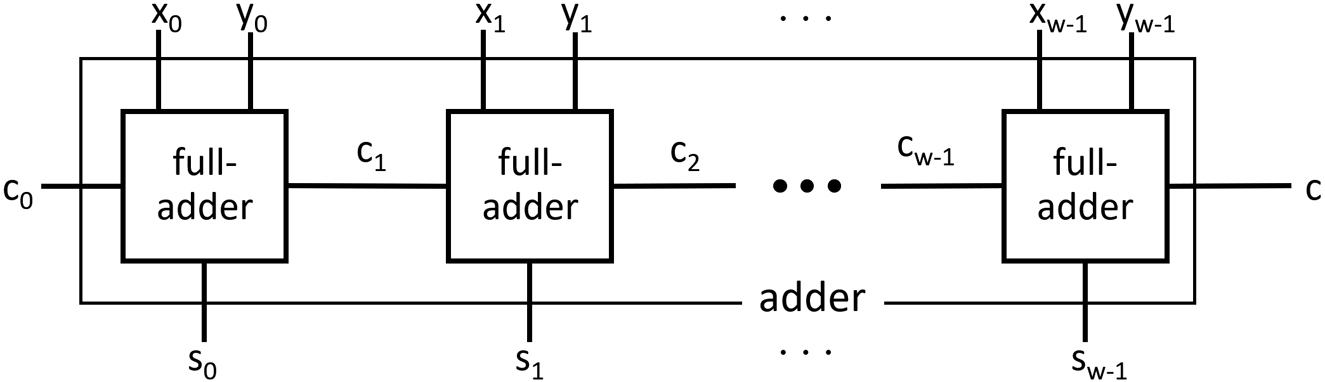
\includegraphics[scale=0.25]{Images/adder.png}
\todo{Improvised with PowerPoint. Redraw using Visio.}
\begin{Verbatim}
(defun adder (c0 x y)
  (if (consp x)
      (let* ((x0 (first x)) (xs (rest x))
             (y0 (first y)) (ys (rest y))
             (a0 (full-adder c0 x0 y0))
             (s0 (first a0)) (c1 (second a0)) ; {add.bit0}
             (a  (adder c1 xs ys))
             (ss (first a)) (c (second a)))   ; {add.bits}
        (list (cons s0 ss) c))                ; {add1}
      (list nil c0)))                         ; {add0}
\end{Verbatim}
\end{center}
\index{equation, by name!\{addo\}, \{add1\}}\index{addition!carry}\index{arithmetic!binary numeral}\index{numeral!binary addition}\index{addition!binary numeral}\index{binary numeral!addition}\index{diagram!ripple-carry circuit}\index{addition!circuit}\index{circuit!addition}\index{circuit!ripple-carry adder}\seeonlyindex{ripple-carry circuit}{circuit}\index{ACL2!circuit model}\index{circuit!ACL2 model}
\caption{Ripple-Carry Adder and ACL2 Model}
\label{fig:adder}
\end{figure}

The ACL2 model in the figure relies
on inductive definition. It feeds the carry-in and
the low-order bits from the two numerals into the \textsf{full-adder} operator.
(The low-order bit in a numeral is the ``ones bit,''
which is the first element of the list that we use to
represent the numeral.)
The sum bit from the list that the \textsf{full-adder} operator delivers
is the low-order bit of the numeral representing the sum of
the numbers that the input numerals represent.
The remaining sum bits in the list are those delivered by
the \textsf{adder} operating on the other bits in the input numerals
(that is, all the bits in the input numerals except the low-order bits).

Because the model defines an operator in ACL2,
you can run the operator to see that it works in specific cases.
To add two binary numerals, supply lists of 0s and 1s
representing those numerals in an invocation
of the \textsf{adder} operator, and specify zero as the input carry-bit.
The output will be binary numeral for the sum.

The theorem in Figure \ref{fig:adder-thm} (page \pageref{fig:adder-thm})
explains how input and output signals are interpreted as numbers.
As with the two-bit adder (Figure \ref{adder2-ok}, page \pageref{adder2-ok})
the three numbers represented by the two input
numerals and the input carry, when added together,
equal the number represented
by a numeral formed from the output sum-bits and
the output carry-bit.
However, the theorem for the \emph{w}-bit adder
is stated as an implication to constrain
inputs to be numerals with the same number of bits.
This was not necessary with the theorem for the two-bit adder
because the lengths of the numerals were explicit in the ACL2 model.

\begin{figure}
\begin{center}
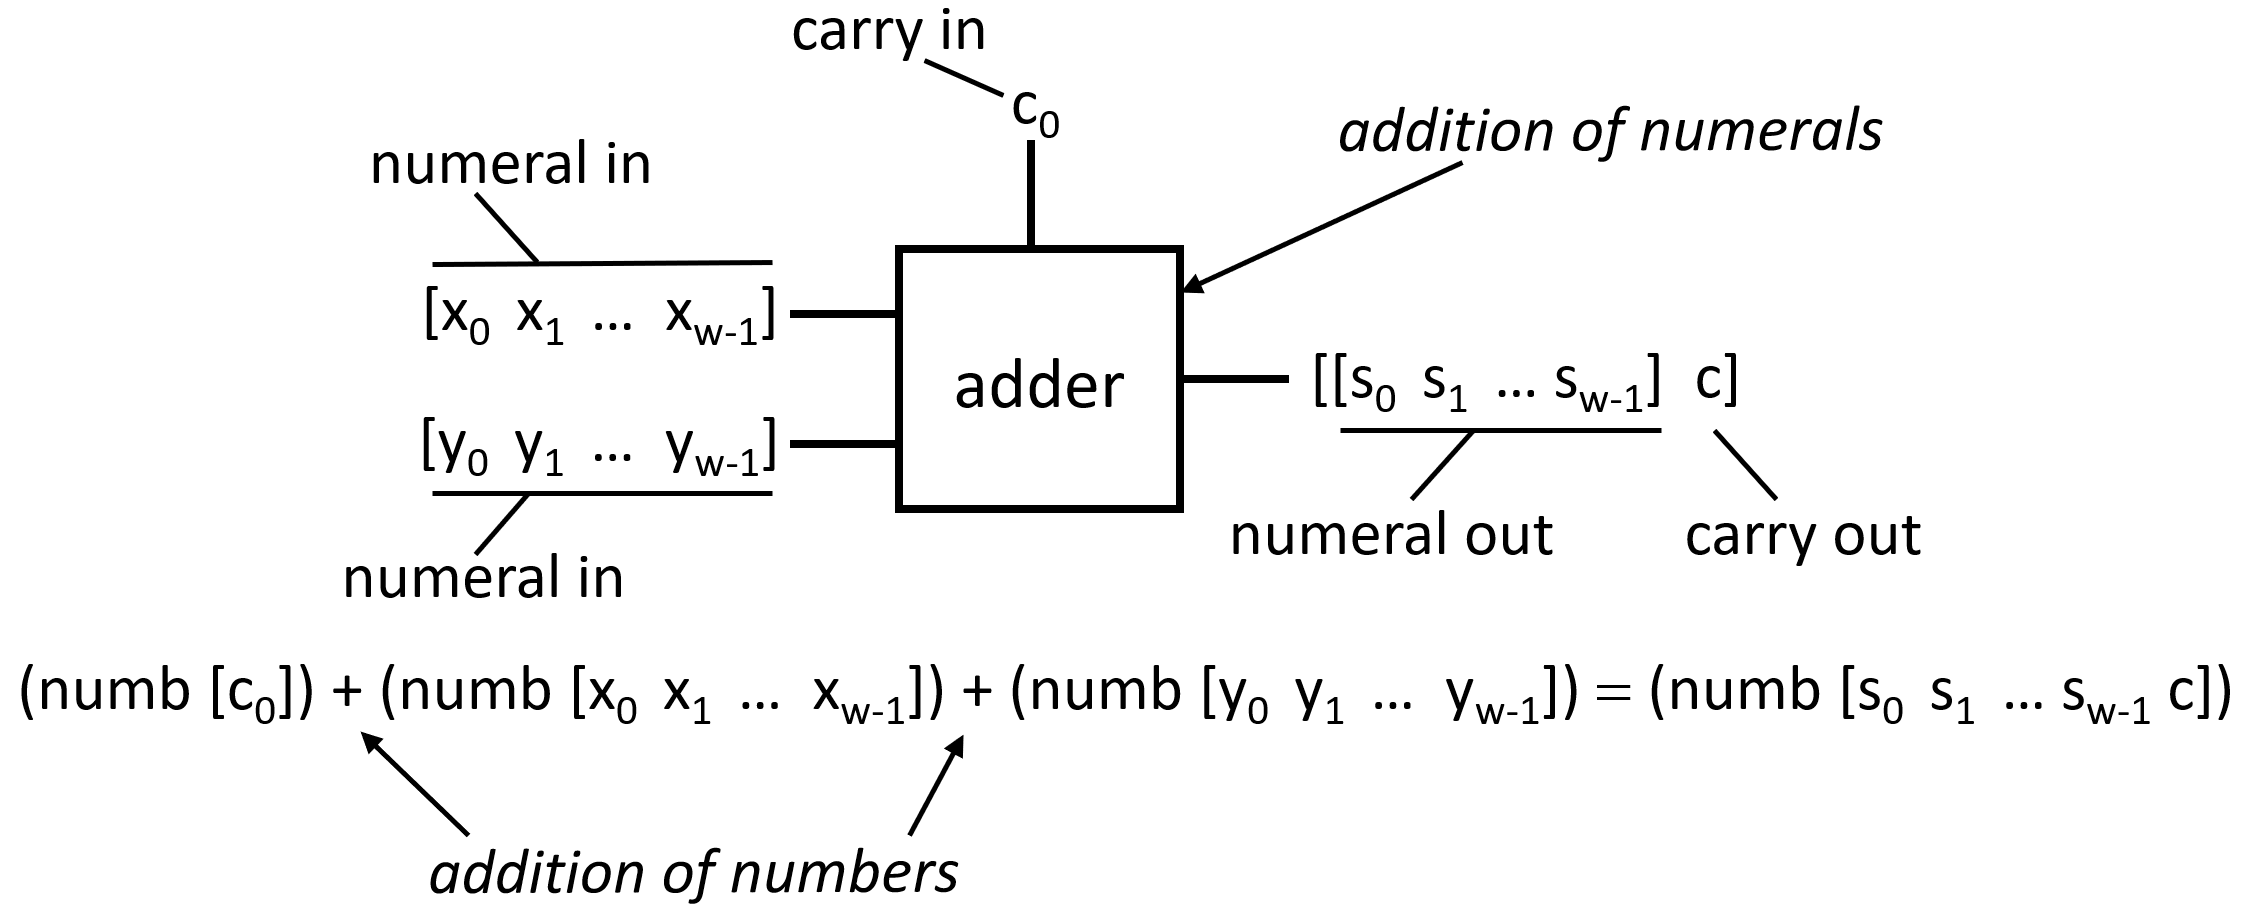
\includegraphics[scale=0.3]{Images/adder-thm.png}
\todo{Improvised with PowerPoint. Redraw using Visio.}
\begin{Verbatim}
(defthm adder-ok
  (implies (= (len x) (len y))
           (let* ((a (adder c0 x y))
                  (s (first a)) (c (second a)))
             (= (numb (append s (list c)))
                (+ (numb (list c0)) (numb x) (numb y))))))
\end{Verbatim}
\end{center}
\seeonlyindex{ripple-carry theorem}{theorem}\index{theorem, by name!\{adder-ok\}}\index{theorem!ripple-carry adder}\index{ACL2!adder-ok}\index{arithmetic!binary numeral}\index{numeral!binary addition}\index{addition!binary numeral}\index{binary numeral!addition}
\caption{Adding \emph{w}-Bit Binary Numerals}
\label{fig:adder-thm}
\end{figure}

Theorem \{adder-ok\} (Figure~\ref{fig:adder-thm}, page \pageref{fig:adder-thm})
states the arithmetic property that we expect the adder circuit to have.
The mechanized logic of ACL2 succeeds in verifying
the theorem without assistance,
but because reasoning about circuits is such an important idea,
we think going through
a paper-and-pencil proof will be worthwhile.
Our proof will, of course, work from
the model of the adder circuit
(Figure \ref{fig:adder}, page \pageref{fig:adder}),
rather than from the circuit diagram.
Aside \ref{circuit-vs-model} (page \pageref{circuit-vs-model})
discusses some of the ramifications of this approach,
which we have used throughout the discussion of circuits.

\begin{aside}
We expect that you could, given a basket of
logic gates, wires, and enough time,
use the diagram of the adder circuit to
build one for any specified word size,
and we think you can convince yourself that the model
matches the diagram.
If it does, then properties of the model
that we verify guarantee that the circuits also have those properties.

In a complete formalization, we would
need a way to convert models into instructions
for fabricating circuits.
The fabricated circuit would have the properties
of the model. Such a formalization
would use the methods we have employed to formalize other operations.
However, in this treatment of the subject
we have left that step to the imagination.
\index{circuit!ACL2 model}\index{model!of circuit}
\caption{Models and Circuit Fabrication}
\label{circuit-vs-model}
\end{aside}
%\begin{samepage}
%\label{adder-thm}\index{theorem, by name!\{adder-ok\}}\index{theorem!ripple-carry adder}\seeonlyindex{ripple-carry theorem}{theorem}\index{numeral!binary addition}\index{addition!binary numeral}\index{binary numeral!addition}
%\begin{center}
%\begin{tabular}{l}
%Theorem \{\emph{adder ok}\} \\
%\textsf{(numb [$s_0$ $s_1$ \dots $s_{n}$ $c$])} $=$
%\textsf{(numb [$c_0$])} $+$ \textsf{(numb [$x_0$ $x_1$ \dots $x_{n}$])} $+$ \textsf{(numb [$y_0$ $y_1$ \dots $y_{n}$])} \\
%where \textsf{[[$s_0$ $s_1$ \dots $s_{n}$] $c$]} $=$ \textsf{(adder $c_0$ [$x_0$ $x_1$ \dots $x_{n}$] [$y_0$ $y_1$ \dots $y_{n}$])}\\
%\end{tabular}
%\end{center}
%\end{samepage}

Figure \ref{fig:adder-thm-prf} (page \pageref{fig:adder-thm-prf})
displays the \{adder ok\} theorem in algebraic notation.
Proving the theorem amounts to
verifying that $(\forall n.R(n))$ is true,
where the predicate $R$, which has the natural numbers as
its universe of discourse, is defined as follows.
\begin{center}
\begin{tabular}{l}
$R(n) \equiv$ $($\textsf{(numb [$s_0$ $s_1$ \dots $s_{n}$ $c$])} $=$\\
\phantom{$R(n) \equiv$ $($}\textsf{(numb [$c_0$])} $+$ \textsf{(numb [$x_0$ $x_1$ \dots $x_{n}$])} $+$ \textsf{(numb [$y_0$ $y_1$ \dots $y_{n}$])}$)$ \\
~~~~~ where \textsf{[[$s_0$ $s_1$ \dots $s_{n}$] $c$]} $=$ \textsf{(adder $c_0$ [$x_0$ $x_1$ \dots $x_{n}$] [$y_0$ $y_1$ \dots $y_{n}$])}\\
\end{tabular}
\end{center}

The proof will use mathematical induction.
Figure~\ref{fig:adder-thm-prf}
displays the equation of the base case, $R(0)$,
and sketches its proof. Here we elaborate some of the details
that were omitted in the sketch.
The first step is
to compute the value of \textsf{(adder $c_0$ [$x_0$] [$y_0$])}
by working through the definition of the \textsf{adder} operator
(Figure \ref{fig:adder}, page \pageref{fig:adder}).
With those operands, the \textsf{if} operator in
the definition of \textsf{adder} selects the \{add1\} equation.
\begin{quote}
\begin{tabular}{rll}
       & \textsf{(adder $c_0$ [$x_0$] [$y_0$])}              & \\
\vspace{1mm}
$=$    & \textsf{[(cons $s_0$ $ss$) $c$]}                    & \{add1\} (page \pageref {fig:adder})  \\
where  &&\\
       & \textsf{[$ss$  $c$]}                                & \\
$=$    & \textsf{(adder $c_1$ (rest [$x_0$]) (rest [$y_0$]))}& \{add.bits\} (page \pageref {fig:adder}) \\
$=$    & \textsf{(adder $c_1$ nil nil)}                      & \{\emph{rst1}\} (page \pageref {rst1}) \\
$=$    & \textsf{[nil  $c_1$]}                               & \{add0\} (page \pageref {fig:adder}) \\
\end{tabular}
\end{quote}
\addtolength{\tabcolsep}{-1mm} 
\begin{tabular}{rll}
Therefore, & $ss$ $=$ \textsf{nil}                                       & \\
           & $c$ $=$ $c_1$                                      & \{$\dagger$\} \\
and        & \textsf{(cons $s_0$ $ss$}) $=$ \textsf{(cons $s_0$ nil)} $=$ \textsf{[$s_0$]} & \{$\ddagger$\}\\
           &                                                    & \\
\end{tabular}\\
\addtolength{\tabcolsep}{1mm}
The equation $R(0)$ (Figure~\ref{fig:adder-thm-prf}) makes the following requirement.
\vspace{1mm}\\
\hspace*{1.5cm}\textsf{[[$s_0$] $c$]} $=$ \textsf{(adder $c_0$ [$x_0$] [$y_0$])}
~~\vspace{2mm}\\
The following argument, which proceeds
from the right-hand side to the left-hand side of the requirement,
confirms that it is consistent with the definition of the \textsf{adder} operator.\\
\begin{tabular}{rll}
 ~~~~~~~~& \textsf{(adder $c_0$ [$x_0$] [$y_0$])} & \\
$=$ & \textsf{[(cons $s_0$ $ss$) $c$]}       & \{add1\}      \\
$=$ & \textsf{[[$s_0$] $c$]}                 & \{$\ddagger$\}\\
\end{tabular}
~~\vspace{2mm}\\
The proof of the base case can be completed as follows.\\
\begin{tabular}{rll}
 ~~~~~~~~& \textsf{(numb [$s_0$ $c$])}                               &                   \\
$=$ & (\textsf{numb [$s_0$ $c_1$])}                             & \{$\dagger$\}    \\
$=$ & \textsf{(numb (full-adder $c_0$ $x_0$ $y_0$))}            & \{add.bit0\}      \\
$=$ & \textsf{(numb [$c_0$])} + \textsf{(numb [$x_0$])} $+$ \textsf{(numb [$y_0$])} & \{full-adder-ok\} \\
\end{tabular}\\

So much for the base case.
Figure~\ref{fig:adder-thm-prf} also presents
a proof of the inductive case: $\forall n.(R(n) \rightarrow R(n+1))$.
When that proof arrives at the sum
\textsf{(numb [$c_1$])} $+$ \textsf{(numb [$x_1$ \dots $x_{n+1}$])} $+$ \textsf{(numb [$y_1$ \dots $y_{n+1}$])},
it recognizes that the induction hypothesis, $R(n)$, applies because
the numerals \textsf{[$x_1$ \dots $x_{n+1}$]} and \textsf{[$y_1$ \dots $y_{n+1}$]} have $n+1$
elements, like the numerals in the equation $R(n)$.
The subscripts run from $1$ to $n+1$ instead of from $0$ to $n$,
but it's the number of bits that counts, not the subscripts.

The induction hypothesis says that this sum equals
\textsf{(numb [$s_1$ \dots $s_{n+1}$ $c$])}, and
the \{\emph{nmb1}\} theorem (Exercise \ref{nmb1}, page \pageref{nmb1})
adds \textsf{(numb [$s_0$])} $+$ $2\times$\textsf{(numb [$s_1$ \dots $s_{n+1}$ $c$])}
to arrive at \textsf{(numb [$s_0$ $s_1$ \dots $s_{n}$ $c$])}.
We have derived the left-hand side
of equation $R(n+1)$, having started from the right-hand side.
That completes the proof of the \{adder ok\} theorem
by mathematical induction.

The proof is tedious, to say the least.
It requires working out the details of
numerous operator invocations
from symbolic representations of the operands.
Fortunately, ACL2 is on hand to work through the
muck and mire and arrive at the same conclusion.
That gives us confidence that our ripple-carry circuit
for adding binary numerals delivers the expected results.

\begin{figure}
Theorem \{adder ok\}\\
$\forall n.($\textsf{(numb [$s_0$ $s_1$ \dots $s_{n}$ $c$])} $=$
\textsf{(numb [$c_0$])} $+$ \textsf{(numb [$x_0$ $x_1$ \dots $x_{n}$])} $+$ \textsf{(numb [$y_0$ $y_1$ \dots $y_{n}$])}$)$\\
\hphantom{(numb}where \textsf{[[$s_0$ $s_1$ \dots $s_{n}$] $c$]} $=$ \textsf{(adder $c_0$ [$x_0$ $x_1$ \dots $x_{n+1}$] [$y_0$ $y_1$ \dots $y_{n}$])}\\
\emph{Base Case}
\begin{center}
\begin{tabular}{l}
\hline
$R(0) \equiv$  $($\textsf{(numb [$s_0$ $c$])} $=$ \textsf{(numb [$c_0$])} $+$ \textsf{(numb [$x_0$])} $+$ \textsf{(numb [$y_0$])}$)$ \\
 ~~~~~~ where \textsf{[[$s_0$] $c$]} $=$ \textsf{(adder $c_0$ [$x_0$] [$y_0$])} \\
\hline
\end{tabular}
\begin{tabular}{ll}
\textsf{(adder $c_0$ [$x_0$] [$y_0$])} $=$ \textsf{[(cons $s_0$ nil) $c$]} $=$ \textsf{[[$s_0$] $c$]} & \{\emph{add1}\} (\{\emph{adder}\} \emph{Fig. \ref{fig:adder}, p.\pageref{fig:adder}}) \\
~~~~ where \textsf{[$s_0$ $c$]} $=$ \textsf{(full-adder $c_0$ $x_0$ $y_0$)}          & \emph{note:} (adder $c$ nil nil) = [nil $c$] \\
\textsf{(numb [$s_0$ $c$])} = \textsf{(numb (full-adder $c_0$ $x_0$ $y_0$)}          &  \\
~~~~~~~~~~~ $=$ \textsf{(numb [$c_0$])} $+$ \textsf{(numb [$x_0$])} $+$ \textsf{(numb [$y_0$])}  & \{\emph{full-adder ok}\} \emph{(Fig. \ref{fig:full-adder-thm}, p.\pageref{fig:full-adder-thm})}\\
\end{tabular}
\end{center}
\emph{Inductive Case}
\begin{center}
\begin{tabular}{l}
 \hline
$R(n+1)$ $\equiv$ $($\textsf{(numb [$s_0$ $s_1$ \dots $s_{n+1}$ $c$])} $=$ \\
\hphantom{$R(n+1)$ $\equiv$ $($}\textsf{(numb [$c_0$])} $+$ \textsf{(numb [$x_0$ $x_1$ \dots $x_{n+1}$])} $+$ \textsf{(numb [$y_0$ $y_1$ \dots $y_{n+1}$])}$)$ \\
 ~~~~~~ where \textsf{[[$s_0$ $s_1$ \dots $s_{n+1}$] $c$]} $=$ \textsf{(adder $c_0$ [$x_0$ $x_1$ \dots $x_{n+1}$] [$y_0$ $y_1$ \dots $y_{n+1}$])} \\
\hline
\end{tabular}
\begin{tabular}{ll}
\hspace*{3mm}\textsf{(numb [$c_0$])} $+$ \textsf{(numb [$x_0$ $x_1$ \dots $x_{n+1}$])} $+$ \textsf{(numb [$y_0$ $y_1$ \dots $y_{n+1}$])}& \\
$=$ \textsf{(numb [$c_0$])} $+$ \textsf{(numb [$x_0$])} $+$ $2\times$\textsf{(numb [$x_1$ \dots $x_{n+1}$])}                         & \{\emph{nmb1}\} \emph{(p. \pageref{nmb1})} \\
\hphantom{$=$ \textsf{(numb [$c_0$])} }$+$ \textsf{(numb [$y_0$])} $+$ $2\times$\textsf{(numb [$y_1$ \dots $y_{n+1}$])}                  & \{\emph{nmb1}\} \\
$=$ \textsf{(numb [$c_0$])} $+$ \textsf{(numb [$x_0$])} $+$ \textsf{(numb [$y_0$])} $+$                                                & \\
 ~~~~~~ $2\times($\textsf{(numb [$x_1$ \dots $x_{n+1}$])} $+$ \textsf{(numb [$y_1$ \dots $y_{n+1}$])}$)$                    & \{\emph{algebra}\} \\
$=$ \textsf{(numb (full-adder $c_0$ $x_0$ $y_0$))} $+$                                                             & \{\emph{full-adder ok}\} \\
 ~~~~~~ $2\times($\textsf{(numb [$x_1$ \dots $x_{n+1}$])} $+$ \textsf{(numb [$y_1$ \dots $y_{n+1}$])}$)$                    & \\
$=$ \textsf{(numb [$s_0$ $c_1$])} $+$ $2\times($\textsf{(numb [$x_1$ \dots $x_{n+1}$])} $+$ \textsf{(numb [$y_1$ \dots $y_{n+1}$])}$)$ & \{\emph{add.bit0}\} \emph{(p.\pageref{fig:full-adder-thm})} \\
$=$ \textsf{(numb [$s_0$])} $+$ $2\times$\textsf{(numb [$c_1$])} $+$                                                          & \{\emph{nmb1}\} \\
\hphantom{$=$ \textsf{(numb [$s_0$ $c_1$])} $+$ }$2\times($\textsf{(numb [$x_1$ \dots $x_{n+1}$])} $+$ \textsf{(numb [$y_1$ \dots $y_{n+1}$])}$)$  & \\
$=$ \textsf{(numb [$s_0$])} $+$                                                                                    & \{\emph{algebra}\} \\
 ~~~~~~ $2\times($\textsf{(numb [$c_1$])} $+$ \textsf{(numb [$x_1$ \dots $x_{n+1}$])} $+$ \textsf{(numb [$y_1$ \dots $y_{n+1}$])}$)$ & \\
$=$ \textsf{(numb [$s_0$])} $+$ $2\times$\textsf{(numb [$s_1$ \dots $s_{n+1}$ $c$])}                                        & \{$R(n)$\} \\
$=$ \textsf{(numb [$s_0$ $s_1$ \dots $s_{n+1}$ $c$])}                                                              & \{\emph{nmb1}\} \\
\end{tabular}
\end{center}
\index{theorem, by name!\{adder-ok\}}\seeonlyindex{adder-ok theorem}{theorem}\index{theorem!ripple-carry adder}\index{numeral!binary addition}\index{addition!binary numeral}\index{binary numeral!addition}\index{arithmetic!binary numeral}
\caption{Theorem \{adder ok\}: Proof by Mathematical Induction}
\label{fig:adder-thm-prf}
\end{figure}

\begin{aside}
A \emph{word} in a computer is a collection of bits
that the computer treats as a whole in certain operations,
such as arithmetic operations.
A circuit to perform arithmetic will carry out
the operation on words denoting binary numerals.
Since all words have the same number of bits,
both of the numerals supplied as inputs to circuit
for an arithmetic operator will have the same number of bits.

We could change the design of the circuit for the adder
to accommodate input numerals of differing lengths.
However, since we are modeling a circuit
in which the input numerals have the same length,
the model does not need to account for that possibility.
\index{word!computer}\index{computer word}
\caption{Adder Circuit and Numerals of Different Lengths}
\label{adder-circuit-and-numerals-of-different-lengths}
\end{aside}

\begin{ExerciseList}
\Exercise \label{ex:add-bin}
Define in ACL2 a operator \textsf{add-bin}
that adds any two binary numerals,
even if the numerals contain a different number of bits.
That is, the value \textsf{(add-bin $c$ $x$ $y$)} should be a binary numeral
for the number \textsf{(numb [$c$])} $+$ \textsf{(numb $x$)} $+$ \textsf{(numb $y$)},
as long as $x$ and $y$ are binary numerals and $c$ is 0 or 1,
regardless of \textsf{(len $x$)} or \textsf{(len $y$)}.
Design and run some sanity checks on your operator.

\Exercise Define in ACL2 a theorem about the operator \textsf{add-bin} (Excercise \ref{ex:add-bin})
that is analogous to theorem \{adder-ok\}
(Figure \ref{fig:adder-thm}, page \pageref{fig:adder-thm}).

\end{ExerciseList}

\section{Numerals for Negative Numbers}
\label{sec:negative-numerals}

So far, all the numerals we've seen have denoted positive numbers.
Arithmetic circuits also need to deal with negative numbers,
and there is more than one way to do that.
The most common scheme is known as the \emph{twos complement} system.

\index{negative numeral}\index{numeral!negative}\index{number!negative}\index{numeral!twos complement}\index{twos complement!numeral}Twos-complement
numerals are a special interpretation of
ordinary binary numerals.
For the numbers $0$, $1$, $\dots$ $(2^{w-1}-1)$,
where \emph{w} is the \emph{word size}
of the circuits for arithmetic operations,
twos-complement numerals are ordinary binary numerals.
All of the numerals for this set of numbers
have $(w-1)$ or fewer bits,
not counting leading zeros
(Theorem \{\emph{len-bits}$\le$\}, page \pageref{len-bitsLE}).
To make the numerals match the word size,
the twos-complement system pads them with leading zeros
to make them have exactly \emph{w} bits.
Leading zeros don't change the number that a numeral denotes
(Theorem \{\emph{leading-0s}\}, page \pageref{leading-0s}), but,
as with the ripple-carry adder (Figure \ref{fig:adder}, page \pageref{fig:adder}),
circuits to perform arithmetic on twos-complement numbers will
require exactly \emph{w} bits for each input numeral
because there are $w$ input lines for each addend,
and each input line must carry a signal.
So, the non-negative numbers, $0$, $1$, \dots $(2^{w-1}-1)$
consume half of the $2^w$ bit-patterns available with
\emph{w}-bit words.

For negative numbers,
the twos-complement system uses the other half of the bit-patterns.
These are the numerals that would normally denote the numbers
$2^{w-1}$, $(2^{w-1}+1)$, \dots $(2^{w}-1)$.
If $(-n)$ is a negative number in the range $-2^{w-1} \leq (-n) < 0$,
\label{2s-def}
then the twos-complement numeral for $(-n)$
is the ordinary binary numeral for $(2^w - n)$.
Since $2^{w-1} = (2^{w}-2^{w-1}) \leq (2^w - n) < 2^w$,
this numeral has exactly \emph{w} bits
(Theorem \{\emph{len-bits}\}, page \pageref{len-bits}).
We also know that its high-order bit is a one-bit
(Theorem \{\emph{hi-1}\}, page \pageref{hi-1}),
so there is an easy way to recognize numerals that denote negative numbers.

For example, a computer with
\index{twos complement!word}\index{word!twos complement}
\index{word!computer}\index{computer word}32-bit words that uses
two-complement numerals has arithmetic circuits that
deal with numbers $n$ in the range $-2^{w-1} \leq n < 2^{w-1}$.
In the positive part of the range, it represents numbers as
ordinary binary numerals, but with enough leading zeros
to fill the 32-bit word.
For a number ($-n$) in the negative part of the range,
the twos-complement system uses the ordinary binary numeral
for the positive number ($2^{32}-n$) to represent the number ($-n$).
Since ($-n$) is in the range
$-2^{31} \leq -n < 0$, we can assert that
$2^{31} \leq 2^{32}-n < 2^{32}$.
Therefore, the twos-complement, binary numeral
for the negative number ($-n$)
has exactly 32 bits (Theorem \{\emph{len-bits}\}, page \pageref{len-bits}).

\index{negative numeral}\index{numeral!negative}\index{number!negative}
\index{numeral!twos complement}\index{twos complement!numeral}
Modular arithmetic makes twos-complement numerals
for negative numbers act like the negative numbers they stand for
when they are added to other numerals.
For negative numbers ($-n$) in the range $-2^{31} \leq -n < 0$,
the value of (($-n$) mod $2^{32}$) is ($2^{32}-n$).
Therefore, since addition and subtraction
in modular arithmetic is consistent with ordinary addition and subtraction
(page \pageref{modular-arithmetic}), it follows that
  ($(m+(-n))$ mod $2^{32}$
= (($m$ mod $2^{32}$) $+$ ($(-n)$ mod $2^{32}$)) mod $2^{32}$
= $((m$ mod $2^{32}$) $+$ $((2^{32} - n)$ mod $2^{32}))$ mod $2^{32}$.

That is, adding the numbers represented by twos-complement
numerals, including numbers in the negative range,
is just like adding ordinary numbers in modular arithmetic.
Subtraction is handled by negating a number
(that is, computing the twos-complement representation
of its negative), then performing addition modulo $2^{32}$.

This method works for any word size.
With word size $w$, the twos complement system
handles addition and subtraction for numbers $n$
in the range $-2^{w-1} \leq n < 2^{w-1}$
by performing ordinary addition of numerals,
as with the ripple-carry adder, but interpreting
the numerals according to the twos-complement scheme.
Circuits for performing addition (and subtraction, which
uses the same circuit in a twos-complement system)
take advantage of the consistency between modular arithmetic
and ordinary arithmetic (page \pageref{modular-arithmetic}).

In summary, the twos-complement representation for computers with
word size $w$ deals with numbers $n$ in the range
$-2^{w-1} \leq n < 2^{w-1}$.
We will refer to this set of integers as $I(w)$.
\label{def-Iw}
\begin{center}
$I(w) = \{-2^{w-1}, \dots -1, 0, 1, 2, \dots 2^{w-1}-1\}$
\end{center}

\index{negative numeral}\index{numeral!negative}\index{number!negative}
\index{numeral!twos complement}\index{twos complement!numeral}
\index{twos complement!word}
Twos-complement numerals for numbers in the negative part of the range
have exactly $w$ bits, with a one-bit in the high-order slot.
Twos-complement numerals for numbers in the positive part of $I(w)$
take the form of ordinary binary numerals, except that
they are padded with enough leading zeros
to fill out a $w$-bit word, where $w$ is the word size of the computer.
The \textsf{twos} operator, defined as follows, delivers the twos-complement numeral
for a number $n$ in the set $I(w)$.

\label{twos-defun}\index{twos complement!operator}\index{operator, by name!twos (twos complment)}\index{operator!twos complement}\index{equation, by name!\{2s$+$\}, \{2s$-$\}}\index{arithmetic!negative numeral}
\begin{Verbatim}
(defun twos (w n)             ; w = word size
  (if (< n 0)                 ; -2^(w-1) <= n < 2^(w-1)
      (bits (+ (expt 2 w) n)) ; {2s-}
      (pad w 0 (bits n))))    ; {2s+}
\end{Verbatim}

The \textsf{twos} operator uses the operator \textsf{bits} (page \pageref{bits-defun})
to compute binary numerals.
For negative numbers it adds $2^w$
(that is, \textsf{(expt $2$ $w$)}, referring to the ACL2 intrinsic operator \textsf{expt})
before computing the numeral.
For non-negative numbers, it computes the numeral,
then uses the \textsf{pad} operator (page \pageref{pad-defun})
to insert leading zeros to match the word-size.
There will always be some padding for numerals representing
positive numbers because
$0 \le n < 2^{w-1}$ implies that
$0 \le $(len (bits $n$)) $< w$
(Theorem \{\emph{len-bits}$\le$\}, page \pageref{len-bitsLE}).

Figure~\ref{fig:2s-comp-3bit} displays
twos-complement numerals for the numbers in the set $I(3)$.
Of course, this example is just to illustrate the idea.
Three is a ridiculously small word size.
No computer would have three-bit words,
but the example gets the point across with a table of manageable size.

\begin{figure}
\begin{center}
\begin{tabular}{cccc}
 $n \in I(3)$ & $2^3+n$  & \textsf{(twos $3$ $n$)}   & \emph{binary numeral} \\
 $-4$         & $4$      & \textsf{[0 0 1]}          & 100                   \\
 $-3$         & $5$      & \textsf{[1 0 1]}          & 101                   \\
 $-2$         & $6$      & \textsf{[0 1 1]}          & 110                   \\
 $-1$         & $7$      & \textsf{[1 1 1]}          & 111                   \\
 $~~0$        &          & \textsf{[0 0 0]}          & 000                   \\
 $~~1$        &          & \textsf{[1 0 0]}          & 001                   \\
 $~~2$        &          & \textsf{[0 1 0]}          & 010                   \\
 $~~3$        &          & \textsf{[1 1 0]}          & 011                   \\
\end{tabular}
\\ $I(w) = I(3) = \{-2^{3-1}=-4, -3, -2, -1, 0, 1, 2, 3=2^{3-1}-1\}$
\\ \emph{word size} $w = 3$
\end{center}
\index{negative numeral}\index{numeral!negative}\index{number!negative}\index{numeral!twos complement}\index{twos complement!numeral}\index{twos complement!word}\index{word!twos complement}\index{arithmetic!negative numeral}
\caption{Twos-Complement Numerals for 3-bit Words}
\label{fig:2s-comp-3bit}
\end{figure}

If the input carry is zero and
the input numerals are interpreted
as twos-complement numerals for numbers in the set $I(w)$,
then the sum-bits of the output numeral from the ripple-carry adder
(Figure \ref{fig:adder}, page \pageref{fig:adder})
form the twos-complement numeral for the sum of the input numerals.
The carry output from the circuit can be used to determine
whether or not the sum is in the set $I(w)$ of numbers representable
by \emph{w}-bit, twos-complement numerals.\footnote{The
output carry can be used to perform multi-word arithmetic
or to detect overflow conditions. Adding two numbers, $m+n$,
that are both in the top half of the positive range
($2^{w-2} \leq m, n < 2^{w-1}$) produces a number that is
outside the set $I(w)$, so the sum has no \emph{w}-bit, twos-complement numeral.
This outcome is known as an overflow.
Similarly, adding two numbers in the bottom half of the
negative range ($-2^{w-1} \leq m,n < -2^{w-2}$)
produces a number outside the twos-complement range, an overflow in the negative direction.}

Now, here is an interesting
\index{negative numeral}\index{numeral!negative}\index{number!negative}\index{numeral!twos complement}\index{twos complement!numeral}\index{twos complement!negation}\index{twos complement!word}\index{word!twos complement}trick
for computing the twos-complement numeral of a negative number without
computing $2^w$ or doing subtraction.
It works like this.
Let \textsf{[$x_0$ $x_1$ \dots $x_{w-1}$]}
be the $w$-bit, binary numeral for a number $n$ in the range $1$, $2$, \dots $2^{w-1}$,
padded if necessary with leading zeros to fill out the $w$-bit word.
Then, the twos-complement numeral for $(-n)$ can be computed
in a two-step procedure.
First, invert the bits: change the zero-bits to one-bits,
and change the one-bits to zero-bits.
Then, use the ripple-carry adder to add the numeral for the number $1$
to the numeral with the inverted bits.
The result will be the twos-complement numeral for $(-n)$.
The same trick works to negate the twos-complement numeral
of a number $(-n)$ from the range $-2^{w-1} < -n \leq 0$.

The trick does not work for the number $-2^{w-1}$
because the negative of that number (namely, $2^{w-1}$)
is outside of the set $I(w)$,
so it doesn't have a \emph{w}-bit, twos-complement numeral.
The trick does work for negating the twos-complement numeral for zero.
In that case the procedure delivers an output numeral identical
to the input (namely, a numeral consisting of \emph{w} zero-bits).
It produces a one-bit for the carry-out, but that bit is not part of the numeral.
Figure~\ref{fig:2s-comp-negation}
(page \pageref{fig:2s-comp-negation})
explains how inverting the bits and adding one leads to the negation
of the input numeral.
It's an exercise in algebra and modular arithmetic.\footnote{The
proof of equation \{$ys$ increment\}
in Figure~\ref{fig:2s-comp-negation}
cites the geometric progression
(Exercise~\ref{ex:geometric-progression}, page \pageref{ex:geometric-progression})}.

\begin{figure}
\emph{Some facts, notation, and equations:}
\begin{center}
\begin{tabular} {ll}
$1 \le n \le 2^{31}$                                   & \emph{range of numbers to negate} \\
\textsf{(len (bits $n$))} $\le w$                               & \{\emph{len-bits}$\le$\} \emph{(page \pageref{len-bitsLE})} \\
$xs$ = {\textsf{[$x_0$ $x_1$ \dots  $x_{w-1}$]}}                & $xs$ = (pad $w$ 0 (bits $n$))\emph{, padded binary numeral} \\
\textsf{(numb $xs$)} = $n$                                      & \{\emph{leading-0s}\} \emph{(page \pageref{leading-0s})} \\
$ys$ = \textsf{[$y_0$ $y_1$ \dots $y_{w-1}$]}                   & \emph{inverted bits} $y_i = 1 - x_i$ \emph{(0s for 1s, 1s for 0s)} \\
$1$ $+$ \textsf{(numb $ys$)} $=$ $2^w - n$                      & \{$ys$ \emph{increment}\} \emph{equation (see proof below)} \\
\textsf{(bits (+ 1 (numb $ys$)))} $=$ \textsf{(twos $w$ $(- n)$)}        & \{\emph{2s trick}\} \emph{equation (see proof below)} \\
\end{tabular}
\end{center}
\emph{Proof of} \{$ys$ \emph{increment}\} \emph{equation:} $1$ $+$ \textsf{(numb $ys$)} $=$ $2^w - n$
\begin{center}
\begin{tabular} {rlcll}
  & $1$   &$+$ &\textsf{(numb $ys$)}                                          &  \\
$=$ & $1$   &$+$ &$y_02^0 + y_12^1 + \dots + y_{w-1}2^{w-1}$                    & \{\emph{Horner 2}\}  \\
$=$ & $1$   &$+$ &$(1 - x_0)2^0 + (1 - x_1)2^1 + \dots ++ (1 - x_{w-1})2^{w-1}$ & $\forall i.(y_i = 1-x_i)$ \\
$=$ & $1$   &$+$ &$(2^0 + 2^1 + \dots + 2^{w-1})$                               & \{\emph{algebra}\}   \\
  &       &$-$ &$(x_02^0 + x_12^1 + \dots + x_{w-1}2^{w-1})$                  &                      \\
$=$ & $1$   &$+$ &$(2^w - 1) - (x_02^0 + x_12^1 + \dots + x_{w-1}2^{w-1})$      & \{\emph{geometric progression}\}\\
$=$ & $2^w$ &$-$ &$(x_02^0 + x_12^1 + \dots x_{w-1}2^{w-1})$                    & \{\emph{algebra}\} \\
$=$ & $2^w$ &$-$ &\textsf{(numb $xs$)}                                          & \{\emph{Horner 2}\}   \\
$=$ & $2^w$ &$-$ &$n$                                                           & \textsf{(numb $xs$)} $=$ $n$     \\
\end{tabular}
\end{center}
\emph{Proof of} \{\emph{2s trick}\} \emph{equation:} \textsf{(bits (+ 1 (numb $ys$)))} $=$ \textsf{(twos $w$ $(- n)$)}
\begin{center}
\begin{tabular} {lll}
    & \textsf{(bits (+ 1 (numb $ys$)))}        & \\
$=$ & \textsf{(bits $(2^w - n)$)}              & \{$ys$ \emph{increment}\} \emph{equation} \\
$=$ & \textsf{(bits $(2^w + (- n))$)}          & \{\emph{algebra}\}                        \\
$=$ & \textsf{(bits (+ (expt 2 $w$) $(- n)$)}) & \emph{ACL2 notation for} $(2^w + (- n))$\\
$=$ & \textsf{(twos $w$ $(- n)$)}              & \{$2s-$\} \emph{(}\{\emph{twos}\}\emph{, page \pageref{twos-defun})} \\
\end{tabular}
\end{center}
\index{arithmetic!negative numeral}\index{negative numeral}\index{numeral!negative}\index{number!negative}\index{numeral!twos complement}\index{twos complement!numeral}\index{twos complement!negation}\index{twos complement!word}\index{word!twos complement}
\caption{Twos-Complement Negation Trick}
\label{fig:2s-comp-negation}
\end{figure}

\begin{ExerciseList}

\Exercise \label{len-2s}\index{twos complement!length}
Prove \{\emph{len-2s}\}:
$\forall w.((n \in I(w)) \rightarrow ($\textsf{(len (twos $w$ $n$))} $= w))$

\Exercise \label{minus-sign}\index{twos complement!sign}
Prove \{\emph{minus-sign}\}:
$\forall w.(((n \in I(w)) \wedge (n < 0)) \rightarrow ($\textsf{(fin(twos $w$ $n$))} $=$ $1))$\\
The operator \textsf{fin} is defined on page \pageref{fin-defun}.

\Exercise \label{plus-sign}\index{twos complement!sign}
Prove \{\emph{plus-sign}\}:
$\forall w.(((n \in I(w)) \wedge (n \geq 0)) \rightarrow ($\textsf{(fin(twos $w$ $n$))} $=$ $0))$

\Exercise \label{2s-negation-circuit}\index{twos complement!negation circuit}
\index{circuit!twos complement negation}
Diagram a negation circuit whose input signals represent a
twos-complement numeral for a number $n$ in the range
$-2^{w-1} < n < 2^{w-1}$
and whose output signals represent
the twos-complement numeral for $(-n)$.
In your diagram, rely on the twos-complement negation trick
(Figure~\ref{fig:2s-comp-negation}),
and use the gate-like symbol in
Figure \ref{fig:adder-thm} (page \pageref{fig:adder-thm})
to depict the ripple-carry adder circuit.\\
\emph{Note}: Your circuit will also produce the twos-complement
numeral for $-2^{w-1}$, given the binary numeral for $2^{w-1}$
as input.

\Exercise \label{2s-negation-circuit-model}
Define an ACL2 model for the negation circuit
of Exercise~\ref{2s-negation-circuit}.
Your model may refer to the ACL2 model
of the ripple carry adder in
Figure \ref{fig:adder} (page \pageref{fig:adder}).

\Exercise Define and run a DoubleCheck property that
tests the ACL2 model of the negation circuit of
Excercise~\ref{2s-negation-circuit-model}.

\Exercise \label{2s-subtraction-circuit}
\index{numeral!subtraction}\index{subtraction, binary numeral}\index{circuit!subtraction}
Diagram a circuit that subtracts twos-complement numerals.
In your diagram, use the gate-like symbol in
Figure \ref{fig:adder-thm} (page \pageref{fig:adder-thm})
to depict the ripple-carry adder circuit,
and use a similar, gate-like symbol for the negation circuit
of Exercise~\ref{2s-negation-circuit}.

\Exercise \label{2s-subtraction-circuit-model}
Define an ACL2 model of the twos-complement
subtraction circuit of Exercise~\ref{2s-subtraction-circuit}.

\Exercise Define and run a DoubleCheck property that
tests the ACL2 model of the subtraction circuit
in Exercise~\ref{2s-subtraction-circuit-model}.

\Exercise \label{2s-comparison-circuit}
\index{circuit!numeric order}\index{number!comparison circuit}\index{compare!circuit, numeric}
Diagram a comparison circuit that takes a pair of
twos-complement numerals as inputs and delivers a one-bit
if the first number is less than the second
and a zero-bit otherwise.
In your diagram, use a gate-like symbol
for the subtraction circuit of Exercise~\ref{2s-subtraction-circuit}.
\emph{Hint}: Apply theorems \{\emph{minus-sign}\} and \{\emph{plus-sign}\}
from Exercises~\ref{minus-sign} and \ref{plus-sign}.

\Exercise \label{2s-comparison-circuit-model}
Define an ACL2 model of the comparison circuit
of Exercise~\ref{2s-comparison-circuit}.
Your model may refer to the subtraction circuit model
of Exercise~\ref{2s-subtraction-circuit-model}.

\Exercise Define and run a DoubleCheck property
that tests the comparison circuit model
of Exercise~\ref{2s-comparison-circuit-model}.

\Exercise \label{ex:geometric-progression}
Use induction prove the following equation. You may assume $r > 0$ and $r \neq 1$.\\
\hspace*{18mm}$(r - 1)(r^0 + r^1 + r^2 + \dots r^n) = r^{n+1} - 1$~~~~~~\{\emph{geometric progression}\}


\end{ExerciseList}

%%% Local Variables:
%%% mode: latex
%%% TeX-master: "book"
%%% End:
